\subsection{Spark [VI]}

Spark is a framework for distributed processing of data \cite{Zaharia2010, Zaharia2013, Spark1, Spark2}.
It works with large datasets and streams of data, and lets to make complex queries on this data.
It consists of two parts: Spark engine that allows to process data in a batch fashion, and Spark streaming that extends Spark engine to handle fast coming streaming data.
Spark is simple, efficient and fault-tolerant.
It abstracts programmer from details of how processing distributes across cluster, and how robustness is achieved.
It shows results that surpass Hadoop in efficiency in 10 times.

Spark has several abstractions to represent data and streams.
Using them it is easy to write simple, short and robust code, that implements complex algorithms on batch and streaming data.
The first one - Resilient Distributed Dataset (RDD) - an object, distributed in the cluster, that contains data to process.
Another one is a Shared Variable - variable, that can be used among the cluster as a counter or a lookup table.
The last abstraction is a Discretized Stream (DStream) - representation of a data stream in a distributed fashion based on RDD objects.
RDDs and shared variables provide basic batch processing framework, whereas DStreams, based on RDDs, allow to process streaming data.

%\subsubsection{Data model and batch processing}

\textit{Resilient Distributed Dataset} \mnote{Resilient Distributed Dataset} (RDD) is the main notion in Spark, that represents dataset in a distributed fashion.
RDD is essentially a readonly collection of elements.
It is fault-tolerant, so that if one partiotion is lost, the whole collection can be recovered.
RDD does not need to exist physically on the cluster nodes.
Instead, it is a lazy object, that can lay in a robust data storage, and be computed on the fly, when computations require particular pieces of data.
Figure~\ref{fig:RDDArchitecture} shows general architecture of an RDD object.

\begin{figure}[h]
  \centering
  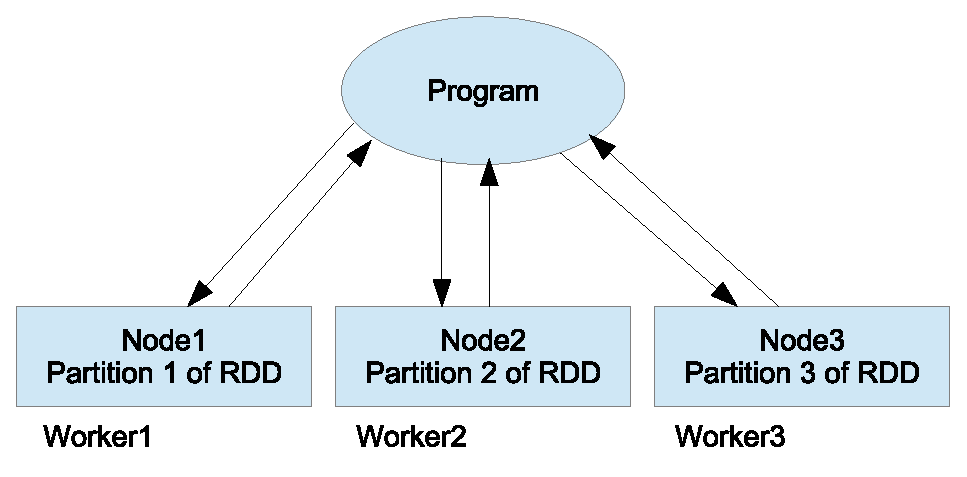
\includegraphics [width=0.7\textwidth]{images/RDDArchitecture}
  \caption{General architecture of an RDD object.}
  \label{fig:RDDArchitecture}
\end{figure}

There are two methods how to obtain an RDD object: parallelizing exisiting collection in the driver program, and using external dataset.
Existing collection is any collection of data, e.g. array, list, set, etc., that is directly handled in the program.
Creating an RDD object in this way, elements of a collection are copied to a distributed dataset, that can be used then in parallel.
It is possible to specify the number of slices, that is the number of tasks, each machine in the cluster will then execute for this collection.
External dataset is an external file.
It can reside in the local file system, and in the distributed file system like HDFS.
The simple example of processing data from the external text file in Spark, is to count the sum of lines' lengths using functions \lstinline{map} and \lstinline{reduce} of an RDD object. 
Additionally, it is possible to obtain RDD by transforming another RDD, or by changing persistance of an existing RDD, but this methods are derived in some sense.

RDD supports two types of operations: transformations and actions.
\textit{Transformation} \mnote{transformation} creates a new RDD object from existing one.
This is useful in many algorithms, because it allows to apply several functions to a dataset one after another.
Examples of transformation are \lstinline{map}, \lstinline{flatMap}, \lstinline{filter}, \lstinline{groupByKey}, \lstinline{reduceByKey}.
For instance, a method \lstinline{map} processes each element of an RDD object using specified function, and returns a new RDD object as a result.
\textit{Action} \mnote{action} executes computations on an RDD object, and returns a value.
Action produces normally a result of the whole algorithm.
Examples of actions are \lstinline{reduce}, \lstinline{collect}, \lstinline{count}, \lstinline{countByKey}.
Method \lstinline{reduce} is a basic example of an action.
It applies specified function to aggregate all elements giving in the RDD object, and returns the resulting value.

Transformation in Spark is a lazy operation, in the sense that it is computed only when action operation requires its result to produce output.
This makes execution more efficient when there is a chain of transformations before final action, because the application does not receive then intermediate RDD objects, but only final resulting value, that is usually much smaller.
Nevertheless, there are cases, when it is to compute different actions on the same transformation.
Then it is meaningful to have RDD object of this transformation computed once, and to have a handle to it in the program.
For this case there is a method \lstinline{persist}, that allows to materialize RDD object.
This is also possible to persist RDD object on disk.

Fault-tolerance of Spark is based on HDFS and on the nature of RDD's realization.
As long as all data locates on HDFS, if any machine fails, all lost data can be recovered.
In case of node failure, RDD recovers itself, so that no data is lost, and processing is going without additional handling of administrator.

To initialize Spark it is first to create a \lstinline{SparkContext} object, that is responsible for a connection of the program to Spark.
It allows to specify properties of the application, and also options of how Spark should run, for example in local mode or on the cluster.
\lstinline{SparkContext} gives an access to different parameters and properties of execution environment.

\begin{lstlisting}[float=h, caption=Counting the total length of all lines in the file using Spark's RDD object., label=listing:RDDExampleCode, language=Java]
SparkConf conf =
		new SparkConf().setAppName(appName).setMaster(master);
JavaSparkContext sc = new JavaSparkContext(conf);
JavaRDD<String> lines = sc.textFile("data.txt");
JavaRDD<Integer> lineLengths = lines.map(s -> s.length());
int totalLength = lineLengths.reduce((a, b) -> a + b);
\end{lstlisting}

On the Listing~\ref{listing:RDDExampleCode} we present a simple program, that counts the sum length of all lines in the text file.
Example is taken from \cite{Spark1}.
Here we create an RDD object from external file, set \lstinline{map} function to count length of the each line, and set \lstinline{reduce} function to sum up lengths of lines.
Execution starts only when \lstinline{reduce} function is called, because, as we discussed, transformations are lazy in Spark.

Normally, passing arguments to a function, that executes on the nodes of the cluster, they are simply copied and there is no feedback to the driver program.
Sometimes it is useful to have global variable or lookup table, that all nodes can access.
Spark supports the notion of a \textit{shared variable}\mnote{shared variable}.
There are two types of shared variables: broadcast variables and accumulators.
\textit{Broadcast variable} \mnote{broadcast variable} represents readonly value or dataset, that is useful for all nodes as a lookup table or global predefined value.
It is copied to every node using method \lstinline{broadcast} of \lstinline{SparkContext}.
There are efficient algorithms in Spark to make this transfer fast.
\textit{Accumulator} \mnote{accumulator} is a distributed counter, that allows all nodes to add up to the global numeric variable.
It can be created using method \lstinline{accumulator} of \lstinline{SparkContext}.
No node can read this value or do anything else than incrementation, what makes its implementation easy and fast.
Only driver program is able to read accumulator's value.

%\subsubsection{Streaming processing}

\textit{Streaming in Spark} \mnote{Spark streaming} is an extension of a Spark engine, described in the previous section.
It can process data stream in a distributed manner.
Spark streaming receives data from the input stream, divides it into blocks, each represented as an RDD, and passes this sequence of blocks to the Spark engine.
It can work with different sources, e.g. message queue server (Kafka), web service (Twitter API), or regular TCP socket.
Processed data can be there stored to the filesystem or database.
The main abstraction for streaming processing in Spark is a Discretized Stream or DStream.
It is internally a sequence of RDDs.
Several DStreams can be combined into one chain for application more complex algorithms. 

\textit{Discretized Stream} or \textit{DStream} \mnote{Discretized Stream (DStream)} is the main abstraction in Spark streaming.
DStream can be the input stream, as well as intermediate stream, generated after processing of input stream of data.
It is essentially a chain of RDD objects, and provides a stream of data, that is to process by Spark.
Each RDD represents batch of data in the period of time, that is specified in the \lstinline{SparkStreamingContext}.
Figure~\ref{fig:SimpleDStream} depicts simple DStream.

\begin{figure}[h]
  \centering
  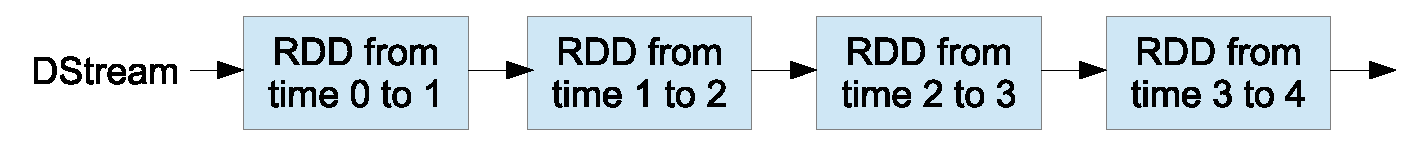
\includegraphics [width=1.0\textwidth]{images/SimpleDStream}
  \caption{Representation of a simple DStream.}
  \label{fig:SimpleDStream}
\end{figure}

Every operation, applied to DStream, is applied to every RDD object in the stream.
This implies, that transformation on the DStream produces new DStream.
All these transformations are executed by Spark engine in a standard batch fashion.
Figure~\ref{fig:DStreamWithTransformation} depicts how it works.

\begin{figure}[h]
  \centering
  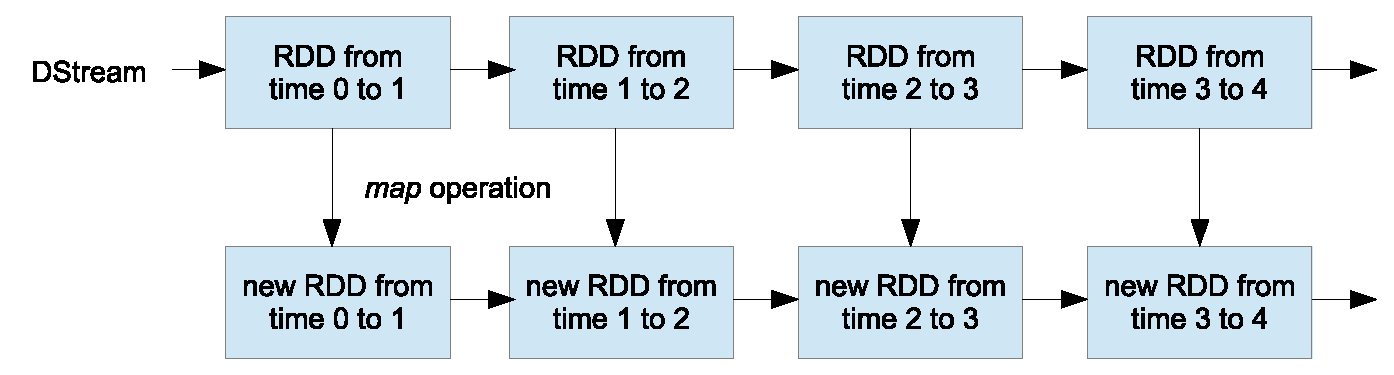
\includegraphics [width=1.0\textwidth]{images/DStreamWithTransformation}
  \caption{Transformation of a DStream to a new DStream.}
  \label{fig:DStreamWithTransformation}
\end{figure}

\textit{Input DStream} is a stream of raw data coming to Spark from the outer source.
Sources can be of two types: basic sources and advanced sources.
Basic sources are sources, that available using standard streaming context API, e.g. files or sockets.
Advanced sources are available using specific libraries, for example Kafka message queue server.
There is a notion of \lstinline{Receiver}, that is an object that receives data from the stream, put into Spark's memory, so that it is available for input DStream, associated with this Receiver.
Every DStream is responsible only for one input data stream.
Many DStreams can be created for different input streams to receive data from different data sources in parallel.
Receiver is executing as a long running task, hence it occupies one core of the processor.
This implies, that there should be more cores then receivers in the system.

There is a list of transformation to apply on a DStream.
They all are almost the same as transformations available for RDD, because DStream works on top of RDD.
The most common are \lstinline{map}, \lstinline{flatMap}, \lstinline{filter}, \lstinline{reduce}, \lstinline{reduceByKey}.

Similarly to Spark engine, it is to create \lstinline{SparkStreamingContext} object to work with Spark streaming.
It allows to adjust environment for processing, set properties like local or cluster mode, number of threads used, and many others.
One important property is the batch interval.
It defines the time of gathering data from the input stream, before creating RDD object and sending it to the Spark engine.

\begin{lstlisting}[float=h, caption={Counting the frequencies of words in the text lines, coming from the TCP socket.}, label=listing:DStreamExampleCode, language=Java]
SparkConf conf = new SparkConf()
		.setMaster("local[2]").setAppName("NetworkWordCount");
JavaStreamingContext jssc =
		new JavaStreamingContext(conf, new Duration(1000));
JavaReceiverInputDStream<String> lines =
		jssc.socketTextStream("localhost", 9999);
JavaDStream<String> words =
		lines.flatMap(line -> Arrays.asList(line.split(" ")));
JavaPairDStream<String, Integer> pairs =
		words.map(w -> new Tuple2<String, Integer>(w, 1));
JavaPairDStream<String, Integer> wordCounts =
		pairs.reduceByKey((x, y) -> x + y);
wordCounts.print();
jssc.start();
jssc.awaitTermination();
\end{lstlisting}

Listing~\ref{listing:DStreamExampleCode} shows a simple example of a Spark streaming program.
Example is taken from \cite{Spark2}.
This code counts frequencies of words coming in a text data from the TCP socket.
First we create \lstinline{SparkStreamingContext} object, and specify it to work in a local mode using two execution threads.
We set a duration of gathering data from the input stream to 1 second.
In the Line 3 we create DStream responsible for an input stream associated with TCP socket.
Then we apply two transformations and one action.
Transformations are \lstinline{map}-functions, so that the first one splits lines to words, and the second transforms words to pairs of the form \lstinline{(word, 1)}.
Action is a \lstinline{reduce} operation that sums up occurances of the same word.
Execution starts only when we call \lstinline{start} method of \lstinline{SparkStreamingContext}.
In the Line 7 we print out partial results of the processing.
Instead, we can push results to a database or to a file, what is usually a case.

Spark streaming has a number of output operations on DStreams, that used to push transformed data to outer systems.
This can be files or databases.
Output operations actually start execution, as \lstinline{actions} of Spark engine do.
Examples of output operations are \lstinline{print}, \lstinline{saveAsObjectFiles}, \lstinline{saveAsTextFiles}, \lstinline{saveAsHadoopFiles}, \lstinline{foreachRDD}.

DStream allows to persist it in the memory, when multiple computations of the same DStream are required.
Method \lstinline{persist} of DStream object does that.
Its execution specifies that every RDD of the DStream will be persisted in the memory, as it is done for RDD in Spark engine.
For data, arriving from network, the persistence level is so, that all data is replicated to two nodes to provide fault-tolerance.

There is a mechanism of checkpointing in Spark streaming, that allows to make snapshots of intermediate data to HDFS.
It is useful in case of \textit{stateful operations} that are executed on multiple batches of data.
They maintain and accumulate metadata, that can be cleaned with checkpoint.
If set not properly, checkpointing makes computation throughput less.
It is advised to set it 5 - 10 times of sliding time.